\documentclass{article}
%packages
\usepackage{graphicx}
\usepackage{hyperref}
\usepackage[utf8]{inputenc}
\usepackage[T1]{fontenc}
\usepackage[frenchb]{babel}
\usepackage[a4paper]{geometry}
\usepackage{minted}

\begin{document}
%title
\begin{titlepage}
	\vspace{-20px}
	\begin{tabular}{l}
		\textsc{Blin} S\'ebastien\\
		\textsc{Collin} Pierre-Henri
	\end{tabular}
	\hfill \vspace{10px}
\includegraphics[scale=0.1]{esir.png}\\
	\vfill
	\begin{center}
		\Huge{\'Ecole sup\'erieure d'ing\'enieurs de Rennes}\\
		\vspace{1cm}
		\LARGE{1\`ere Ann\'ee}\\
		\large{Parcours Informatique}\\
		\vspace{0.5cm}\hrule\vspace{0.5cm}
		\LARGE{\textbf{Algorithmie et complexité}}\\
		\Large{Compte-Rendu TP4}
		\vspace{0.5cm}\hrule
		\vfill
		\vfill
	\end{center}
	\begin{flushleft}
		\Large{Sous l'encadrement de~:}\\
		\vspace{0.2cm}
		\large{{Ridoux} Olivier}\\
		\large{{Maurel} Pierre}
	\end{flushleft}
	\vfill
\end{titlepage}

\section{Algorithme génétique : KS}
\subsection{Objectif}
Dans la première partie de ce TP, nous allons étudier le problème du sac à dos. Pour cela, nous allons utiliser le principe d'algorithme génétique. Le problème est représenté par une liste de poids, un tableau de booléen qui renvoie true si le poids i est présent dans le sac, ainsi qu'une capacité maximale. Le but étant de maximiser le nombre de poids qu'on peut mettre dans un sac sans dépasser sa capacité maximale.
\subsection{Moyens mis en \oe uvre}
On a commencé par compléter la classe Individu_SAD qui réprésente un individu dans le cadre du problème du sac à dos.
\begin{minted}{java}
boolean[] _individu = null;
double[] _weights = null;
double _capacite = 0;

public Individu_SAD(double[] weights, double capacite)
{
	_weights = weights;
	_capacite = capacite;
	_individu = new boolean[weights.length];
	Random random = new Random();
	for(int i = 0; i < weights.length; ++i)
		_individu[i] = random.nextBoolean();
}

/**
 * renvoie l'adaptation de cet individu
 */
public double adaptation()
{
	double adapt = 0;
	for(int i = 0; i < _individu.length; ++i)
		if(_individu[i])
			adapt += _weights[i];
	if(adapt > _capacite)
		return 0;
	return adapt;
}

public boolean[] getIndividu()
{
	return _individu;
}
\end{minted}
Pour le croisement de deux individus, on choisit un indice au hasard et on inverse les sous-chaines.
\begin{minted}{java}
/**
 * renvoie un tableau de 2 individus constituant les
 * enfants de la reproduction entre this et conjoint
 * @param conjoint à accoupler avec l'objet courant
 * @return tableau des 2 enfants
 */
public Individu[] croisement(Individu conjoint)
{
	Individu_SAD[] crois = new Individu_SAD[2];
	boolean[] res = new boolean[_individu.length];
	boolean[] res2 = new boolean[_individu.length];
	int index = 0;
	Random random = new Random();
	index = random.nextInt(_individu.length-1);
	for(int i = 0; i < index; ++i)
	{
		res[i] = _individu[i];
		res2[i] = ((Individu_SAD)conjoint)._individu[i];
	}	
	for(int i = index + 1; i < _individu.length; ++i)
	{
		res[i] = ((Individu_SAD)conjoint)._individu[i];
		res2[i] = this._individu[i];
	}
	crois[0] = new Individu_SAD(_weights, _capacite);
	crois[1] = new Individu_SAD(_weights, _capacite);
	crois[0]._individu = res;
	crois[1]._individu = res2;
	return crois;
}

/**
 * applique l'opérateur de mutation
 * associé à la probabilité prob
 */
public void mutation(double prob)
{
	for(int i = 0; i < _individu.length; ++i)
		if(Math.random() < prob)
			_individu[i] = !_in
}
\end{minted}
Ensuite, nous avons complété la classe population qui réprésente un ensemble d'individus.
\begin{minted}{java}
private List<Indiv> population;

/**
 * construit une population à partir d'un tableau d'individu
 */
Population(Indiv[] popu){
	population = new LinkedList<Indiv>();
	for(Indiv i : popu)
		population.add(i);
}

/**
 * sélectionne un individu (sélection par roulette par exemple, cf TD)
 * @param adapt_totale somme des adaptations de tous 
 * les individus (pour ne pas avoir à la recalculer)
 * @return indice de l'individu sélectionné
 */
public int selection(double adapt_totale){
	while(true)
	{
		int i = (int)Math.random()*population.size();
		if(Math.random() 
		   < population.get(i \% population.size()).adaptation()/adapt_totale)
			return i;
	}
}

/**
 * remplace la génération par la suivante
 * (croisement + mutation)
 * @param prob_mut probabilité de mutation
 */
@SuppressWarnings("unchecked")
public void reproduction(double prob_mut) {
	
	/***** on construit la nouvelle génération ****/
	List<Indiv> new_generation = new LinkedList<Indiv>();
	
	/* élitisme */
	new_generation.add(individu_maximal());

	double adapt = 0;
	for(Indiv i : population)
		adapt += i.adaptation();
	// tant qu'on n'a pas le bon nombre 
	while (new_generation.size()<population.size()){
		// on sélectionne les parents
		Indiv p1 = population.get(selection(adapt));
		Indiv p2 = population.get(selection(adapt));
		
		// ils se reproduisent
		Individu[] enfants = p1.croisement(p2);
		
		// on les ajoute à la nouvelle génération
		for(int i = 0; i < enfants.length; ++i)
			new_generation.add((Indiv) enfants[i]);
	}
	
	// on applique une éventuelle mutation à toute la nouvelle génération
	boolean first = true;
	for(Indiv i : new_generation)
		if(!first)
		i.mutation(prob_mut);
		else
		first = false;

	//on remplace l'ancienne par la nouvelle
	population = new_generation;
}

/**
 * renvoie l'individu de la population ayant l'adaptation maximale
 */	
public Indiv individu_maximal(){
	Indiv max = null;
	double maxScore = 0;
	for(Indiv i : population)
		if(i.adaptation() > maxScore)
		{
			max = i;
			maxScore = i.adaptation();
		}
	return max;
}

/**
 * renvoie l'adaptation moyenne de la population
 */
public double adaptation_moyenne(){
	double adapt = 0;
	for(Indiv i : population)
		adapt += i.adaptation();
	return adapt/population.size();
}

/**
 * renvoie l'adaptation maximale de la population
 */	
public double adaptation_maximale(){
	return individu_maximal().adaptation();
}
\end{minted}
Enfin, pour tester l'algorithme nous avons complété la classe Client_Sac_A_Dos.
\begin{minted}{java}
public static void main(String[] args){
	
	/* paramètres */ 
	int nbr_indiv=100;
	double prob_mut=0.1;
	
	/* On initialise les poids en lisant un fichier 
	 */
	
	int nbr_objets=28;
	int capacite=1581;
	
		int nbr_objets=70;
		int capacite=350;		
	
	double[] poids = charge_poids("../data_sad/nbrobj"+nbr_objets+"_capacite"+capacite+".txt",nbr_objets);
	
	
	/* on crée une population (aléatoire)
	 * de nbr_indiv individus de taille nbr_objets
	 */
	Individu_SAD[] pop = new Individu_SAD[nbr_indiv];
	for(int i = 0; i < nbr_indiv; ++i)
		pop[i] = new Individu_SAD(poids, capacite);
	Population _p = new Population(pop);

	
	/* on génére les générations successives
	 * en faisant se reproduire la population
	 * et on affiche l'adaptation moyenne et maximale de chaque génération
	 * on s'arrête si on a atteint la capacité ou si on fait un nombre donné (paramètre) d'itérations
	 * le résultat est alors donné par l'individu maximal de la dernière génération
	 */
	int it = 0;
	double best = -1;
	while(it < 10000 && best < capacite)
	{
		System.out.println("Génération " + it);
		System.out.println("Adaptation moyenne : " + _p.adaptation_moyenne());
		System.out.println("Adaptation maximale : " + _p.adaptation_maximale());
		_p.reproduction(prob_mut);
		best = _p.individu_maximal().adaptation();
		++it;
	}
	
	boolean[] val= ((Individu_SAD)_p.individu_maximal()).getIndividu();
		System.out.println("Résultat : ");
	for(boolean b : val)
		System.out.print(b?"1":"0");
	System.out.println("\nAvec un score de :"+_p.individu_maximal().adaptation());
}
\end{minted}
\subsection{Résultats}
Pour tester l'algorithme, nous avons utilisé deux jeux de données : le premier nous donne nombre d'objets = 28 et capacite = 1581. Après plusieurs essais, nous atteignons les solutions suivantes : \\
- en 5 itérations (1001011000101001000100101111)
- en 21 itérations (0101100110100101011000001000)
- en 12 itérations (1101101010101101000101100001)
Globalement, le résultat s'atteint dans un ordre d'une dizaine d'itérations. Le deuxième jeu de données nous donne : nombre d'objets = 70, capacite = 350. Après plusieurs essais, nous avons trouvé les résultats suivants :\\
- 183 itérations (1111111110111111111111111111111111110101111111110111111110111111111111\\
- 314 itérations (0111111111110111111111111111111111111111111111111111111011111111111111\\
- 119 itérations (1111111110111111111101110111111111111111111111111111111110111111011111)\\
- 232 itérations (1111111111111111101100111111111111111110111111111111111110111111111111)\\
). De façon générale, le résultat est atteignable avec un ordre de grandeur d'une centaine d'itérations.
\section{Conclusion}
On constate que l'utilisation d'algorithme génétique permet d'obtenir une solution satisfaisante assez rapidement même avec un nombre important d'objets.
\section{Algorithme génétique : TSP}
\subsection{Objectif}
Dans la seconde partie de ce dernier TP, nous avons utilisé l'algorithme génétique précédement implémenté (en ne modifiant que la partie client et la représentation interne de l'individu) afin de résoudre un problème assez différent, le problème du voyageur de commerce.\\
Dans ce problème, les données nous fournissaient des coordonnées de villes (x,y). Le but était alors de trouver le chemin le plus court passant par tous les points décrit par les données fournies.

\subsection{Moyens mis en \oe uvre}
Pour résoudre ce problème, nous avons gardé la classe Population utilisée dans le problème KS, même si d'autres méthodes existent (\url{http://endomorphis.me/blog/2013/10/11/modele-de-parallelisme-en-iles-pour-des-metaheuristiques/}, \url{http://en.wikipedia.org/wiki/Genetic_algorithm}, etc.). En effet, la méthode de sélection ainsi que de reproduction fonctionne exactement de la même manière pour le problème du voyageur de commerce et pour le problème du sac à dos.\\
Pour ce qui s'agit de la partie client, nous avons repris l'algorithme du précédent client, que nous avons un peu modifié pour qu'il fonctionne avec nos individus.
\begin{minted}{java}
/* parametres */ 
int nbr_indiv=100;
double prob_mut=0.008;
int nbr_villes = 64;
double[] coord_x = new double[nbr_villes];
double[] coord_y = new double[nbr_villes];
charge_coords("../data_vdc/"+nbr_villes+"coords.txt",nbr_villes, coord_x, coord_y);
Individu_VDC[] pop = new Individu_VDC[nbr_indiv];
for(int i = 0; i < nbr_indiv; ++i)
	pop[i] = new Individu_VDC(coord_x, coord_y);
Population _p = new Population(pop);

/* on genere les generations successives
 * en faisant se reproduire la population
 * et on affiche l'adaptation moyenne et maximale de chaque generation
 * on s'arrete si on a atteint la capacite ou si on fait un nombre donne (parametre) d'iterations
 * le resultat est alors donne par l'individu maximal de la derniere generation
 */
int it = 0;
double best = -1;
Display_VDC disp = new Display_VDC((Individu_VDC)_p.individu_maximal());
while(it < 1000)
{
	System.out.println("generation " + it);
	_p.reproduction(prob_mut);
	best = 1/((Individu_VDC)_p.individu_maximal()).adaptation();
	System.out.println("Score : " + best);
	if(it%50 == 0)
		disp.refresh((Individu_VDC)_p.individu_maximal());
	++it;
}
disp.refresh((Individu_VDC)_p.individu_maximal());
int[] val= ((Individu_VDC)_p.individu_maximal()).get_parcours();
System.out.println("Resultat : ");
for(int b : val)
	System.out.print(b);
System.out.println("\nAvec un score de :"+_p.individu_maximal().adaptation());
\end{minted}
Pour la représentation interne, un tableau d'entier nous paraissait le plus facile à manipuler. L'individu contient donc un tableau d'entier représentant l'ordre dans lequel le voyageur visite les villes. À la création, le tableau et intialisé dans un ordre aléatoire avec des numéros entre 0 et le nombre de villes -1.
\begin{minted}{java}
private double[] _x;
private double[] _y;
private int[] _ind;

//Constructeur
public Individu_VDC(double[] coord_x, double[] coord_y) {
	_x = coord_x;
	_y = coord_y;
	_ind = new int[_x.length];
	for(int i = 0; i < _ind.length; ++i)
		_ind[i] = i;
	shuffleArray(_ind);
}

public static void shuffleArray(int[] a) {
	int n = a.length;
	Random random = new Random();
	random.nextInt();
	for (int i = 0; i < n; i++) {
		int change = i + random.nextInt(n - i);
		swap(a, i, change);
	}
}
\end{minted}
L'adaptation consiste à calculer la longueur du trajet. Dans ce cas, plus le score est minimal, plus la réponse est bonne. Et comme miniser revient à maximiser son inverse, on considère 1/la longueur du trajet.\\
\begin{minted}{java}
@Override
public double adaptation() {
	double adapt = 0;
	for(int i = 1; i < _ind.length; ++i)
		adapt += Math.abs(Math.sqrt(Math.pow(_x[_ind[i-1]]-_x[_ind[i]],2)+Math.pow(_y[_ind[i-1]]-_y[_ind[i]],2)));
	return 1/adapt;
}
\end{minted}
Pour le croisement, nous avions le choix entre plusieurs algorithmes. Nous avons hésité entre le croisement ordinal et celui proposé sur \url{http://labo.algo.free.fr/pvc/algorithme_genetique.html}. Nous avons implémenté le second car nous ne l'avions pas encore vu en cours.
\begin{minted}{java}
@Override
public Individu[] croisement(Individu conjoint) {
	Individu[] res = new Individu[1];
	Individu_VDC ind = new Individu_VDC(_x,_y);
	int index = 0;
	Random random = new Random();
	index = random.nextInt(_ind.length-1);
	//On copie la premiere partie du parent 1
	for(int i=0; i<_ind.length; ++i)
		ind._ind[i] = -1;
	for(int i=0; i<=index; ++i)
		ind._ind[i] =_ind[i];
	++index;
	for(int i=0; i<_ind.length; ++i)
	{
		boolean p = false;
		for(int t : ind._ind)
			if(t == ((Individu_VDC)conjoint)._ind[i])
				p = true;
		if(!p)
		{
			ind._ind[index]=((Individu_VDC)conjoint)._ind[i];
			++index;
		}
	}
	res[0] = ind;
	return res;
}
\end{minted}
Enfin pour la partie mutation, nous avons décidé qu'elle serait modélisée par un échange de 2 villes.
\begin{minted}{java}
@Override
public void mutation(double prob) {
	for(int i = 0; i < _ind.length; ++i)
		if(Math.random() < prob)
		{
			int r = (int)(Math.random()*((double)_ind.length));
			int temp = _ind[r];
		_ind[r] = _ind[i];
			_ind[i] = temp;
		}
}
\end{minted}

\subsection{Résultats}
Nous avons alors testé notre algorithme sur des données pour 4, 16, 64 et 250 villes. On remarque que l'algorithme génétique donne rapidement de bons résultats (voir le meilleur résultat) pour un nombre assez faible de ville. À partir de 64 villes, il devient difficile de trouver de meilleurs résultats, l'algorithme commence à converger vers une solution différente de la meilleure solution.\\
Nous remarquons qu'il faut alors passer par d'autres méthodes. Il est possible de choisir d'autres méthodes de reproduction par exemple ou encore mieux, trouver une optimisation ! En effet, à la fin du cours, nous avons vu qu'avec une petite optimisation (que nous n'avons pas implémenté) de commencer avec un score très proche de 12 dès le début de l'algorithme. (11 étant la meilleure solution).\\
On peut voir les résultats 	de notre algorithme avec les figures suivantes.\\
\begin{figure}
	\begin{center}
		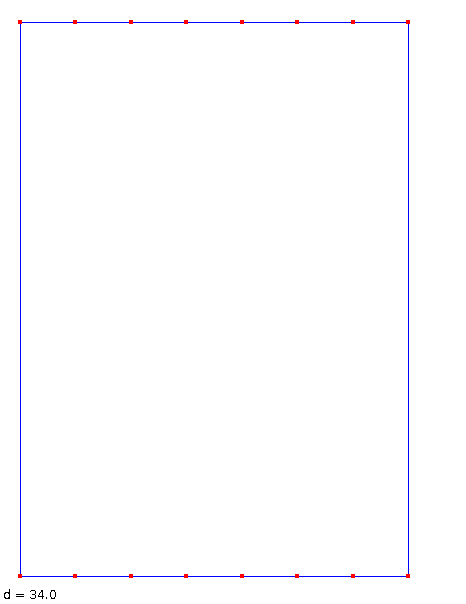
\includegraphics[scale=0.7]{images/16-32gen}\\
		Solution pour 16 villes, après 32 générations
	\end{center}
\end{figure}
\begin{figure}
	\begin{center}
		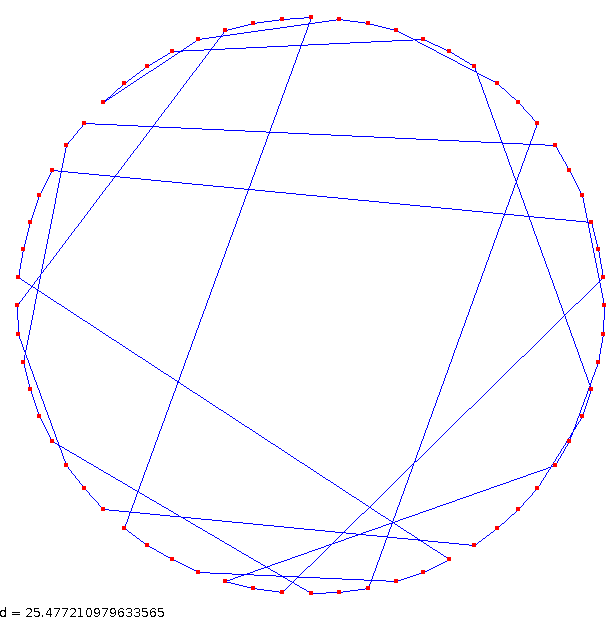
\includegraphics[scale=0.7]{images/64-1000gen}\\
		Solution pour 64 villes, après 1000 générations
	\end{center}
\end{figure}
\begin{figure}
	\begin{center}
		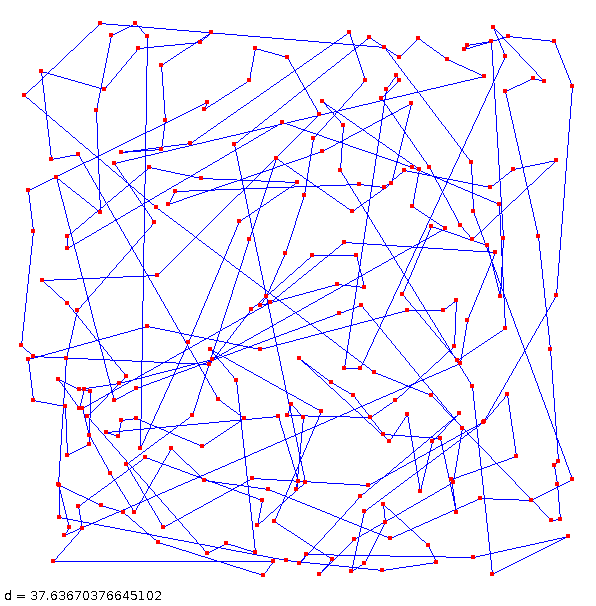
\includegraphics[scale=0.7]{images/250-1000gen}\\
		Solution pour 250 villes, après 1000 générations
	\end{center}
\end{figure}
\section{Conclusion}
On peut donc voir que l'algorithmie génétique est un outil très puissant qui permet de trouver rapidement des solutions convenables à des problèmes compliqués comme KS, TSP, etc. Mais généralement, une optimisation est nécessaire pour tirer pleinement profit de ce type de méthode. En effet, dans le cas de TSP, pour un nombre important de villes, l'algorithme a du mal à trouver une bonne solution lorsqu'il part de rien. Il nécessite alors des optimisations pour pouvoir converger vers une meilleure solution. 
\end{document}

